\documentclass{llncs}
%%%%%%%%%%%%%%%%%%%%%%%%%%%%%%%%%%%%%%%%%%%%%%%%%%%%%%%%%%%
%% package sillabazione italiana e uso lettere accentate
\usepackage[latin1]{inputenc}
\usepackage[english]{babel}
\usepackage[T1]{fontenc}
%%%%%%%%%%%%%%%%%%%%%%%%%%%%%%%%%%%%%%%%%%%%%%%%%%%%%%%%%%%%%

\usepackage{url}
\usepackage{xspace}

\usepackage{float}

\makeatletter
%%%%%%%%%%%%%%%%%%%%%%%%%%%%%% User specified LaTeX commands.
\usepackage{manifest}

\makeatother


%%%%%%%
 \newif\ifpdf
 \ifx\pdfoutput\undefined
 \pdffalse % we are not running PDFLaTeX
 \else
 \pdfoutput=1 % we are running PDFLaTeX
 \pdftrue
 \fi
%%%%%%%
 \ifpdf
 \usepackage[pdftex]{graphicx}
 \else
 \usepackage{graphicx}
 \fi
%%%%%%%%%%%%%%%
 \ifpdf
 \DeclareGraphicsExtensions{.pdf, .jpg, .tif}
 \else
 \DeclareGraphicsExtensions{.eps, .jpg}
 \fi
%%%%%%%%%%%%%%%
 
\newcommand{\java}{\textsf{Java}}
\newcommand{\contact}{\emph{Contact}}
\newcommand{\corecl}{\texttt{corecl}}
\newcommand{\medcl}{\texttt{medcl}}
\newcommand{\msgcl}{\texttt{msgcl}}
\newcommand{\android}{\texttt{Android}}
\newcommand{\dsl}{\texttt{DSL}}
\newcommand{\jazz}{\texttt{Jazz}}
\newcommand{\rtc}{\texttt{RTC}}
\newcommand{\ide}{\texttt{Contact-ide}}
\newcommand{\xtext}{\texttt{XText}}
\newcommand{\xpand}{\texttt{Xpand}}
\newcommand{\xtend}{\texttt{Xtend}}
\newcommand{\pojo}{\texttt{POJO}}
\newcommand{\junit}{\texttt{JUnit}}

\newcommand{\action}[1]{\texttt{#1}\xspace}
\newcommand{\code}[1]{{\small{\texttt{#1}}}\xspace}
\newcommand{\codescript}[1]{{\scriptsize{\texttt{#1}}}\xspace}

% Cross-referencing
\newcommand{\labelsec}[1]{\label{sec:#1}}
\newcommand{\xs}[1]{\sectionname~\ref{sec:#1}}
\newcommand{\xsp}[1]{\sectionname~\ref{sec:#1} \onpagename~\pageref{sec:#1}}
\newcommand{\labelssec}[1]{\label{ssec:#1}}
\newcommand{\xss}[1]{\subsectionname~\ref{ssec:#1}}
\newcommand{\xssp}[1]{\subsectionname~\ref{ssec:#1} \onpagename~\pageref{ssec:#1}}
\newcommand{\labelsssec}[1]{\label{sssec:#1}}
\newcommand{\xsss}[1]{\subsectionname~\ref{sssec:#1}}
\newcommand{\xsssp}[1]{\subsectionname~\ref{sssec:#1} \onpagename~\pageref{sssec:#1}}
\newcommand{\labelfig}[1]{\label{fig:#1}}
\newcommand{\xf}[1]{\figurename~\ref{fig:#1}}
\newcommand{\xfp}[1]{\figurename~\ref{fig:#1} \onpagename~\pageref{fig:#1}}
\newcommand{\labeltab}[1]{\label{tab:#1}}
\newcommand{\xt}[1]{\tablename~\ref{tab:#1}}
\newcommand{\xtp}[1]{\tablename~\ref{tab:#1} \onpagename~\pageref{tab:#1}}
% Category Names
\newcommand{\sectionname}{Section}
\newcommand{\subsectionname}{Subsection}
\newcommand{\sectionsname}{Sections}
\newcommand{\subsectionsname}{Subsections}
\newcommand{\secname}{\sectionname}
\newcommand{\ssecname}{\subsectionname}
\newcommand{\secsname}{\sectionsname}
\newcommand{\ssecsname}{\subsectionsname}
\newcommand{\onpagename}{on page}

\newcommand{\xauthA}{Roberto Casadei}
\newcommand{\xauthB}{NameB StudentB}
\newcommand{\xauthC}{NameC StudentC}
\newcommand{\xfaculty}{II Faculty of Engineering}
\newcommand{\xunibo}{Alma Mater Studiorum -- University of Bologna}
\newcommand{\xaddrBO}{viale Risorgimento 2}
\newcommand{\xaddrCE}{via Venezia 52}
\newcommand{\xcityBO}{40136 Bologna, Italy}
\newcommand{\xcityCE}{47023 Cesena, Italy}

%
% Comments
%
\newcommand{\todo}[1]{\bf{TODO:}\emph{#1}}

\setcounter{secnumdepth}{3}
\setcounter{tocdepth}{3}

\begin{document}

\title{Convoy Cruise Control}

\author{\xauthA}

\institute{%
  \xunibo\\\xaddrCE, \xcityCE\\\email{roberto.casadei12@studio.unibo.it}
}

\maketitle

\begin{abstract}
\footnotesize
This document represents a snapshot of the development process of the Convoy Cruise Control.

%MANIFEST
%\category{I.2.5}{Artificial Intelligence}{Programming Languages and Software}
%\category{I.2.11}{Artificial Intelligence}{Distributed Artificial Intelligence}[Intelligent Agents]

%\terms{Agent programming languages; Methodologies and Languages}

%\keywords{Environment programming in Multi-Agent Systems, Action/perception models, Agent Programming Languages}

\keywords{Convoy Cruise Control, control system, development process, requirements, analysis, project, implementation, testing.}
\end{abstract}

\sloppy

%===========================================================================
\section{Introduction}
\labelsec{intro}
%===========================================================================

\subsection{Vision}


\subsection{Goals}

%===========================================================================
\section{Requirements}
\labelsec{Requirements}
%===========================================================================

Look at \url{www.cruisecontrolsystem.it/requirements.pdf}

%===========================================================================
\section{Requirement analysis}
\labelsec{ReqAnalysis}
%===========================================================================



\subsection{Glossary}
\begin{itemize}
  \item \emph{CONVOY CRUISE CONTROL}: It is a control system that allows to manage the convoy and the convoy's vehicles. It receives the information from the vehicles about their status and speed, and send commands to them, allowing to monitor and control the behavior of the overall convoy and of the single vehicles.\\

  \item \emph{CONVOY}: It is a line of vehicles with a chief at the head.\\

  \item \emph{VEHICLE}: It is a means of conveyance which is able to move autonomously. It must keep a precise position in the line and move at the \emph{speed} which has been set by the chief. It includes a dashboard with a display that shows the current speed (in Kms/sec and Kms/h) and the number of kilometers covered by the vehicle.\\

  \item \emph{CHIEF VEHICLE}: It is the vehicle on which the chief (the person responsible for the convoy) stays. It has a dashboard which is composed of a display that shows the status of all the convoy's vehicles and of a display like that of the other vehicles. Moreover, the chief vehicles has a control panel that allows to set the convoy speed and to make it start and stop. Through the dashboard and the control panel, the chief can interface himself to the Cruise Control System. \\

  \item \emph{DASHBOARD}: It is a panel that contains displays which allow to see multiple information. \\

  \item \emph{DISPLAY}: It is something that can render some textual content.\\

  \item \emph{CONTROL PANEL}: It is a panel which contains buttons and input fields. It allows to send commands to the convoy's vehicles upon a certain communication infrastructure.\\

  \item \emph{KILOMETER COUNTER}: It's needed by the vehicles in order to keep the count of the kilometers covered.\\

\end{itemize}

\subsection{Use Cases}

\begin{figure}
   \centering
   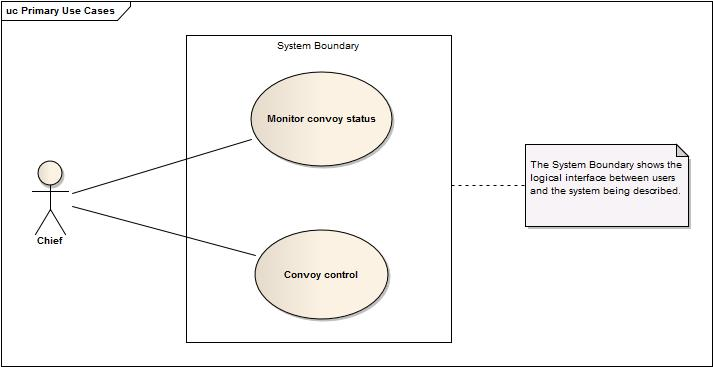
\includegraphics[scale = 0.5]{../Diagrams/Primary_Use_Cases.jpg}\\
  \caption{Primary use cases}\labelfig{testTypes}
\end{figure}

\subsection{Scenarios}
The following scenarios express the main things we want the system to do. 

\begin{table}[H]
\caption{Scenario 1: Monitor Convoy Status}
\label{tab:Scenario1}
\begin{tabular}{| p{2cm} | p{10cm} |}
\hline
\bf{Field} & \bf{Description}\\[3pt]
\hline
ID(Nome) & UC1 - Monitor Convoy Status\\[3pt]
\hline
Description & Here the chief monitors the status of all the vehicles of the convoy.\\[1pt]
\hline
Actors & Chief.\\[3pt]
\hline
Main scenario & The chief will look the display in the chief vehicle's dashboard and will see one flag for each vehicle in the convoy, indicating if the vehicle is able or not to run. These flags are set by the Convoy Cruise Control according to the information gathered from the vehicles.\\[3pt]
\hline
Preconditions & A convoy must exist and a communication infrastructure must be up and running.\\[3pt]
\hline
Postconditions & If one vehicle is able to run, its flag must be green, red otherwise.\\[3pt]
\hline
\end{tabular}
\end{table}

\begin{table}[H]
\caption{Scenario 2: Convoy Control}
\label{tab:Scenario1}
\begin{tabular}{| p{2cm} | p{10cm} |}
\hline
\bf{Field} & \bf{Description}\\[3pt]
\hline
ID(Nome) & UC2 - Convoy Control\\[3pt]
\hline
Description & Here the chief controls the convoy's vehicles through a dashboard on the chief vehicle at the head of the convoy.\\[1pt]
\hline
Actors & Chief.\\[3pt]
\hline
Main scenario & The chief wants to make the convoy start. In order to do so, he will \emph{set the speed} of the convoy (i.e. of all the convoy's vehicles) and then will send a \emph{start} command.\\[3pt]
\hline
Secondary scenarios & Sometimes, when the convoy is running, the chief may decide to stop it. In order to do so, he will send to the convoy a \emph{stop} command.\\[3pt]
\hline
Preconditions & A convoy must exist and a communication infrastructure must be up and running. In order to send a \emph{start} command, the convoy speed must be set.\\[3pt]
\hline
Postconditions & All the convoy's vehicles must execute the command sent by the chief, if possible.\\[3pt]
\hline
\end{tabular}
\end{table}

\newpage
\subsection{Domain Model}

\subsubsection{The Convoy Cruise Control} $\\$
The following interfaces summary the operations that need to be performed by the Convoy Cruise Control. The CCC encapsulates the convoy control logic.

\begin{figure}
   \centering
   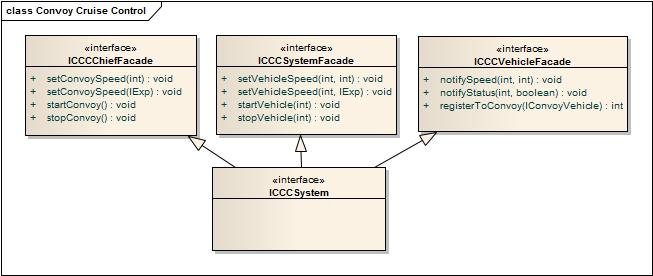
\includegraphics[scale = 0.6]{../Diagrams/Domain_Model_ICCC.jpg}\\
  \caption{Domain Model - The CCC system}\labelfig{testTypes}
\end{figure}

For a semantic description of the \emph{Convoy} entity, look at the \emph{ConvoyTest} test case.

\subsubsection{The Vehicle} $\\$

\begin{figure}
   \centering
   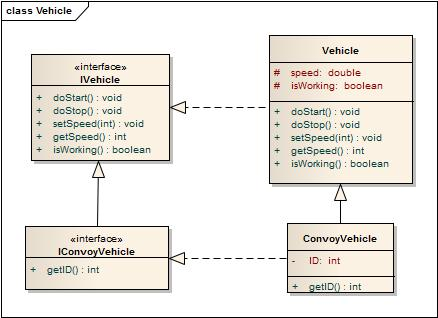
\includegraphics[scale = 0.5]{../Diagrams/Domain_Model_Vehicles.jpg}\\
  \caption{Domain Model - Vehicles}\labelfig{testTypes}
\end{figure}

For a semantic description of this entity, look at the \emph{TestVehicle} test case.

\subsubsection{The Chief Vehicle} $\\$

The chief vehicle is just a vehicle. In addition, it is equipped with a dashboard that allows it to interface with the CCC.

%
%\begin{figure}
%   \centering
%   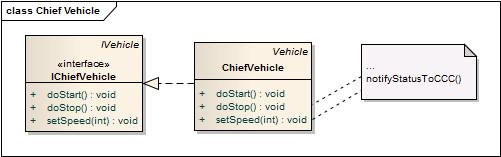
\includegraphics[scale = 0.5]{../Diagrams/Domain_Model_ChiefVehicle.jpg}\\
%  \caption{Domain Model - Chief Vehicle}\labelfig{testTypes}
%\end{figure}

%For a semantic description of this entity, look at the \emph{TestChiefVehicle} test %case.

%\subsubsection{The Convoy} $\\$
%
%\begin{figure}
%   \centering
%   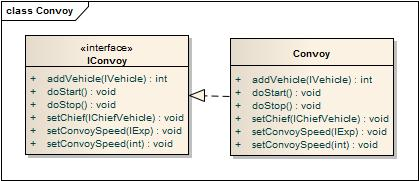
\includegraphics[scale = 0.7]{../Diagrams/Domain_Model_Convoy.jpg}\\
%  \caption{Domain Model - Convoy}\labelfig{testTypes}
%\end{figure}

%For a semantic description of this entity, look at the \emph{TestConvoy} test case. 

\subsubsection{Dashboard, Display, Command Panel and Kilometer Counter} $\\$

The Display and Kilometer Counter entities has been already modelled in a previous project ( see \emph{The Kilometer Counter} ).$\\$
The same argument applies for the dashboard (which is a frame that is able to host multiple displays and buttons), the command panel and the I/O communication infrastructure.$\\$

We'll leverage on these well-proved solutions in order to strike down the cost and time of the project.\\


\newpage
%===========================================================================
\section{Problem analysis}
\labelsec{ProblemAnalysis}
%===========================================================================

\subsection{Main Issues}
\subsubsection{Convoy construction} $\\$
A convoy is composed of at least two vehicles, with the first one being the chief.

\subsubsection{Vehicle Identification} $\\$
The vehicles \emph{and} their position need to be identified.

\subsubsection{Convoy Management} $\\$
Some issues need to be considered when it has to do with the management of the convoy.

\begin{itemize}
  \item When a convoy has to be started, the \emph{start} commands have to be sent from the first vehicle to the last one; moreover, they have to be sent spaced with a delay that allows to guarantee a security distance of \emph{DD} m.
  \item When a convoy has to be stopped, the \emph{stop} commands have to be sent from the last vehicle to the first one; otherwise, a pile-up crash is possible.


\end{itemize}

%When the vehicles need to communicate their status and speed to the CCC system, they need a way to refer to themshelves.

%It turns out that the vehicles must keep a precise position in the convoy, which can be seen as a line of vehicles with a chief vehicles at the head. So, \emph{we can identify the vehicles by their position in the line}.\\
%This identification number can be provided when the vehicles register themshelves to the convoy.\\
%Alternatively, a name or ID can be associated to the vehicles when they're constructed, and this name is passed when they're registered to the convoy.\\
%At the present, we'll adopt the former alternative.

\subsection{Distribution}
The Convoy Cruise Control is intrinsically a distributed system. Consequently, the notion of CCC is distributed along the system: the vehicles and the chief vehicle has to be aware of it.\\

\subsection{Logical Architecture}

\subsubsection{Structural View} $\\$

\begin{figure}
   \centering
   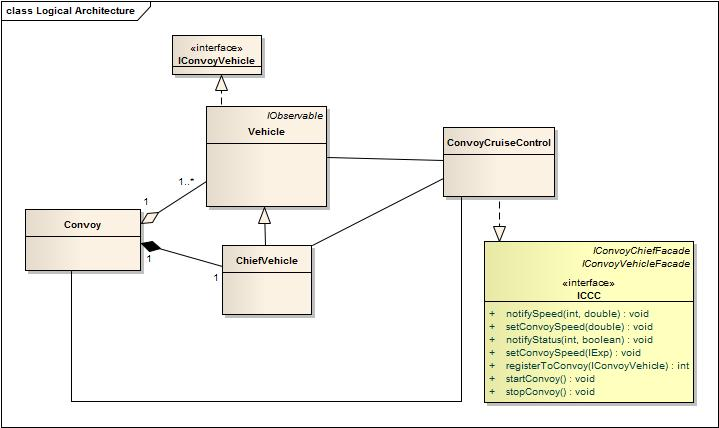
\includegraphics[scale = 0.5]{../Diagrams/Logical_Architecture.jpg}\\
  \caption{Logical Architecture - Structural View}\labelfig{testTypes}
\end{figure}

\subsubsection{Interaction View} $\\$

\begin{figure}
   \centering
   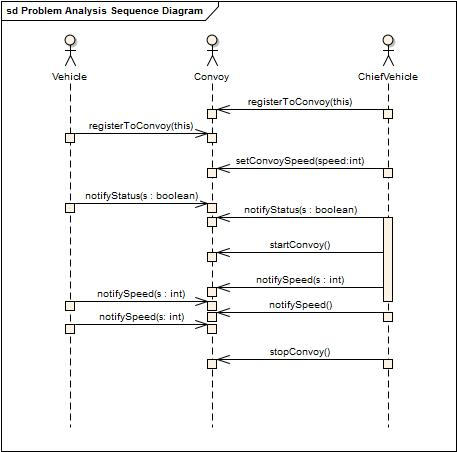
\includegraphics[scale = 0.6]{../Diagrams/Problem_Analysis_Sequence_Diagram.jpg}\\
  \caption{Logical Architecture - Interaction View}\labelfig{testTypes}
\end{figure}

%===========================================================================
\section{Project}
\labelsec{Project}
%===========================================================================

\subsection{Structure}
\subsection{Interaction}
\subsection{Behavior}

%===========================================================================
\section{Implementation}
\labelsec{Implementation}
%===========================================================================

%===========================================================================
\section{Deployment}
\labelsec{Deployment}
%===========================================================================
 
\newpage
%===========================================================================
\section{Notes (outside the template)}
\labelsec{Notes}
%===========================================================================
We report here some general consideration for the next lab:
\begin{itemize}
  \item The solution to a problem defines \textbf{\emph{how}} we achieve some goal (how we design and implement a software system that satisfies the requirements).
  \item Before presenting \emph{how} we achieve a goal, we must explicitly define \textbf{\emph{what}} must be achieved.
  \item If we want to verify that our code works as it is expected, we must define \emph{what is expected} (e.g. by means of a set of \emph{testing plan}).
  \item  To be sure that all the tests are performed, all the test should be done in \emph{automatic} way each time we modify the code.
 \end{itemize}

%===========================================================================
\section{Testing}
\labelsec{testing}
%===========================================================================
\begin{itemize}
  \item \emph{Black box testing}: testing on the target public API without knowledge of the target source code
  \item \emph{White box testing}: testing with knowledge of the target source code
\end{itemize}

\begin{figure}
    \centering
   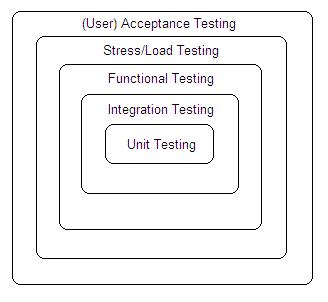
\includegraphics[scale = 0.7]{img/tests.JPG}\\
  \caption{Test types}\labelfig{testTypes}
\end{figure}

\begin{itemize}
  \item \emph{Unit Testing}: testing single units of work
  \item \emph{Integration Testing}: testing how different units of work interact
  \item \emph{Functional Testing}: testing subsystems (usually on a boundary API)
  \item \emph{Stress/Load Testing}: testing the system performance
  \item (\emph{User) Acceptance Testing}: testing the system as a user
\end{itemize}


%===========================================================================
\section{Next steps overview}
\labelsec{next}
%===========================================================================
\begin{enumerate}
  \item Requirement analysis: from names to entities and from verbs to actions.
  \item The concept of \emph{application domain}.
  \item ''What to do'' :  \texttt{IContaKm}, an interface that sets a standard.
  \item ''What is expected'' : black-box  \emph{unit testing plans}.
  \item Problem analysis: a fundamental step to face the risks and to find critical aspects. The interaction problem: methods vs. messages.
  \item Problem analysis: a fundamental step (for a company or a project team) to define a \emph{working plan}.
  \item The (\pojo) \texttt{ContaKm} as a organism: the concept of invariant.
  \item A first main question: is platform-independent (technology-independent) design possible?
  \item The project of the structure and behavior of the (\pojo) \texttt{ContaKm}.
   \item A logic classification of the operations: \emph{primitives, selectors,...}
  \item The problem of a \texttt{display} for the \texttt{ContaKm}.
  \item The implementation of the (\pojo) type \texttt{ContaKm}. Reusing available resources: the case of a (cyclic) \texttt{Counter}.
  \item Automatic testing of the final unit via \junit.
\end{enumerate}


\appendix


\bibliographystyle{abbrv}
\bibliography{biblio}

\end{document}












